% Standalone TikZ figure (compile to PDF/SVG for embedding in Markdown).
\documentclass[tikz,border=2pt]{standalone}
\usepackage{tikz}
\usepackage{xcolor}
\usetikzlibrary{arrows.meta,positioning,matrix}

\begin{document}
\pagecolor{white}\color{black}
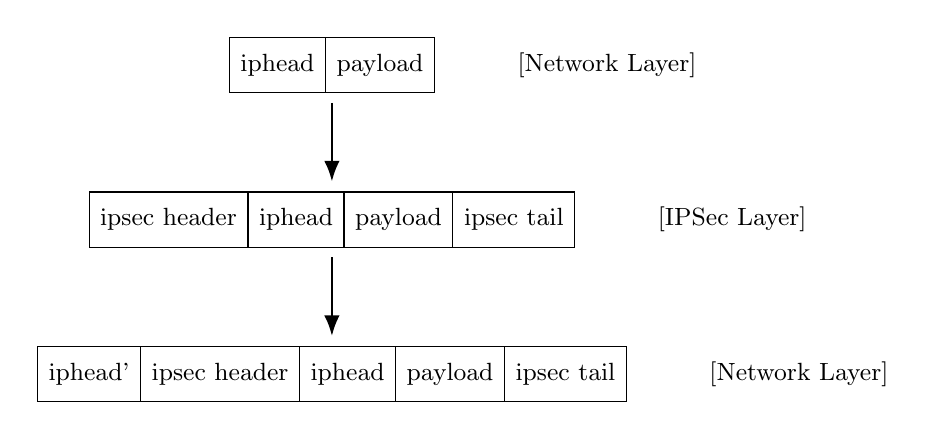
\begin{tikzpicture}[
  token/.style={draw, rectangle, minimum height=7mm, inner xsep=4pt, inner ysep=2pt, outer sep=0pt, font=\small},
  label/.style={font=\small, text=black},
  flow/.style={-Latex, line width=1pt, draw=black},
  % column sep is slightly negative so adjacent borders visually merge.
  row/.style={matrix of nodes, nodes={token}, row sep=0pt, column sep=-0.4pt},
]

% Network layer (original packet)
\matrix[row] (p0) {
  iphead & payload \\
};
\node[label, right=8mm of p0.east] (p0lbl) {[Network Layer]};

% IPSec layer (encapsulated packet)
\matrix[row, below=10mm of p0] (p1) {
  ipsec header & iphead & payload & ipsec tail \\
};
\node[label, right=8mm of p1.east] (p1lbl) {[IPSec Layer]};

% Network layer (outer IP header added)
\matrix[row, below=10mm of p1] (p2) {
  iphead' & ipsec header & iphead & payload & ipsec tail \\
};
\node[label, right=8mm of p2.east] (p2lbl) {[Network Layer]};

\draw[flow] (p0.south) -- (p1.north);
\draw[flow] (p1.south) -- (p2.north);

\end{tikzpicture}
\end{document}
